% Introdu��o
\chapter{Introduction}

The goal of this chapter is to present the technical concepts for a better understanding of our job. 


\section{Cloud Computing}

Technology evolved with big steps over the last decades. Internet is now a pervasive concept and individuals can be connected virtually everywhere on Earth. \cite{Armbrust09m.:above}

Web applications and IT-based processes followed this evolution and today almost every company rely on software on its production chain. Information Technology can be a competitive advantage of a company, but it \textbf{might not}  be part of its core business\cite{powell1997information}. In fact, this is a common scenario on most of the successful companies of the current century.

To avoid losing track of its core business, a number of companies now prefer to outsource (part of) their IT department to other companies \cite{quinn2013technology}. In other words, today it is possible to outsource IT infrastructure, product development and even the entire IT department to other companies.

In the late 60's, former Stanford University professor John McCarthy \cite{DBLP:journals/cacm/McCarthy67} introduced the concept of time-sharing of computing services. In fact, Mr. McCarthy believed that computer resources would be provided as commodities, like water and electricity. 

Several years later, this concept brought to life the notion of \textit{Cloud Computing}, together with new concepts, such as Infrastructure as a Service \textit{(IAAS)}, Platform as a Service \textit{(PAAS)}, Software as a Service \textit{(SAAS)} and Everything as a Service \textit{(XaaS)}~\cite{AViewOfCloudComputing}.

According to~\cite{AViewOfCloudComputing}, \textit{Cloud computing refers to both the applications delivered as services over the Internet and the hardware and systems software in the data centers that provide those services.} 


\section{Everything as a Service - XaaS}

Service-Oriented Architecture (SOA) defines several concepts of ``as-a-service'' models. To enumerate a few, it is possible to find mentions to Platform as a Service (PaaS), Infrastructure as a Service (IaaS), Software as a Service (SaaS), Database as a Service (DBaaS), Desktop as a Service (DaaS), Monitoring as a Service (MaaS) and Communication as a Service (CaaS) on the literature. 

To summarize all these concepts, a new term arose: Everything as a service (XaaS)\cite{7214098}.

On the context of Cloud Computing, however, three of them are the most relevant, and we define more precisely below:

\begin{itemize}
   \item{Infrastructure as a service (IaaS): It is the most simple kind of ``as-a-service'' product and is located on the base of the IaaS-PaaS-SaaS Stack - Figure ~\ref{fig:cloudstach}. IaaS mostly refers to (Virtual) Machines, Storage Devices, Network Infrastructure and other infrastructural services that are available on Cloud Computing vendors.}
   \item{Platform as a Service (PaaS): PaaS refers to the development environment that are available from cloud vendors. It is composed by a development stack, and generally offers databases, web servers and execution runtime. Examples of PaaSs are Amazon BeanStalk, Microsoft Azure and Google AppEngine.  }
   \item{Software as a Service (SaaS): Software as a Service refers to the complex software that runs on the cloud: Webmail, CRM, Gaming Platforms, Learning Management Systems, etc. SaaSs, just as IaaSs and PaaSs generally charge its' users a monthly/yearly fee. The fee is generally conceived in a pay-as-you-go model, so users get charged in a scalable way.  
}

\end{itemize}

\begin{figure}[ht!]
\centering
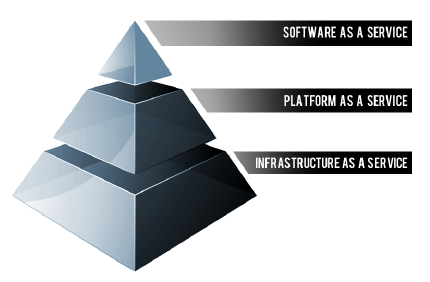
\includegraphics[width=80mm]{cloud_stack.png}
\caption{IaaS-PaaS-SaaS Stack~\cite{kepes2011understanding}.\label{fig:cloudstach}}
\end{figure}


\section{The technological shift}
The adoption of cloud solutions is growing fast among organizations~\cite{6546068}.
Centralized (mostly mainframe) technology is being replaced by distributed and more flexible forms of data storage and processing.
This change of paradigm is motivated by the necessity to improve the use of resources, as well as by the increasing velocity in which data is produced.

On the early 90's it was commonplace for every Information Technology (IT) company to have its own Data Center with huge servers and mainframes. 
IT costs were high, and high-performance computing was available only for big companies, as data centers required a large physical infrastructure and have high costs for maintenance~\cite{Armbrust09m.:above}.

The regular way of building a web application was to use a client-server approach, where the server was a powerful (and expensive) machine. 
At the same time, new players, such as Google or Yahoo, were rising with bigger missions: \textit{``to organize the world's information and make it universally accessible and useful''}~\cite{Spector:2012:GHA:2209249.2209262}. 
The popularization of the internet use incentivized new ways of commerce exchange, yielding an explosion in the amount of data produced and exchanged. 
It was \textit{just} impossible to store the petabytes of daily-generated data in a single server. 

From this point on, the community realized the economical convenience of building and maintaining several low-performance servers, instead of a single high-performance one, even if this this requires a change of culture in the administration of the new datacentres. The new approach (scale-out) is also incompatible with the traditional way of building applications (scale-up), that usually were designed to work on a single server and database. Both approaches are represented on Figure~\ref{fig:scaleupout}

\begin{figure}[ht!]
\centering
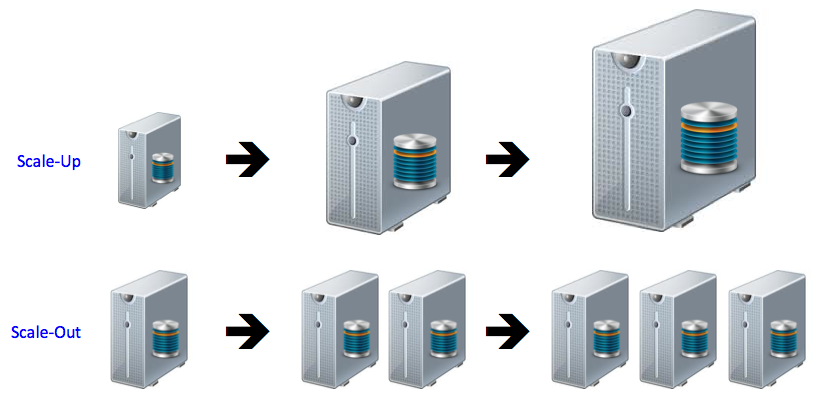
\includegraphics[width=100mm]{scaleOut.png}
\caption{Scale Out vs Scale Up.\label{fig:scaleupout}}
\end{figure}


Several research initiatives were conducted in this area and a common solution was rising: to distribute data storage and processing. 
Google, Yahoo and other big IT players helped to build open source tools to make this approach possible, like Hadoop~\cite{5496972}.



\section{Data Integration, NoSQL Movement \& Polyglot Persistence}
On the last years, the number of Data Base (DB) Engines grew like never before~\cite{dbranking}. 
Along with the NoSQL (Not only SQL) movement and expansion of Social Networks, new concepts for Database Models appeared, like Document Store, Search Engines, Key-Value store, Wide Column Store, Multi-Model and Graph DBMS. 
In~\cite{dbranking} a ranking of the most popular DB engines is presented.

Today, instead of having a single Relational Database Management System (DBMS) for the whole application, it is efficient and cost-effective to have several Data Base Engines, one for each type of data that the application handles. 
This concept is called \textit{Polyglot Persistence}~\cite{sadalage2012nosql}.

As \cite{AdressingDataManagementCloud} illustrates, polyglot persistence is very useful in the context of  e-commerce applications that deal with a catalog, user access logs, financial information, shopping carts and purchase transactions, for example.
The notion of polyglot persistence is built upon the observation that the \textit{nature} of each data type is significantly different (i.e: user logs imply high volume of writes on multiple nodes, shopping carts need high availability and user sessions require rapid access for reads and writes). 

As computing services started to decentralize, developers started to build applications that depended of several data-sources. 
By this time the use of Web Services and Service Oriented Architecture (SOA) became more popular~\cite{Armbrust09m.:above}. 



\section{Transitioning Processes}

In 1965 Gordon E. Moore, Intel's co-founder, published a paper stating that the number of components in integrated circuits had doubled every two years, and would continue to do so for the at least another decade  \cite{658762}.

A similar trend is stablished for commercial software. Wirth's law, Gates' law (Microsoft) or Page's law (Google) state that ``the speed of software halves every 18 months'', compensating Moore's law. \cite{wirth1995a}\cite{brinbreaking}

In other words, software components evolve as well as hardware evolves. Useful software are usually versioned, updated and patched on a regular basis. As stated by \cite{922739}, maintaining software products is not cheap, and generally consumes on average 60\% of software costs.

Time-to-market (TTM) is the length of time that takes for from a product being conceived until its' available for sale. Minimum-Viable-Product (MVP) is the product with the highest return on investment versus risk \cite{blank2013four}. Building a MVP and selling it should be the primary goal of a startup \cite{blank2013four}. 

The current economy demands faster shipping of software products in order to meet the desired TTM of software products and to deploy MVPs in less time. Cloud computing and Agile Methods made software development and deployment faster, cheaper and easier for a number of companies. 

One of the points of the 12 principles of the Agile Manifesto \cite{fowler2001agile} is \textit{``Deliver working software frequently, from a couple of weeks to a couple of months, with a preference to the shorter timescale''}.

This need for speed on software delivery has its' downsides, however. Decisions must be made by the IT department on a short time schedule, sometimes leaving not enough time to make the best choices on the technologies that should be used on a software product. This and other factors oftenly leads to a software migration, replacement or transitioning scenario. In this scenario (part of) a software is replaced with a more suitable alternative.

In the context of Service-Oriented Architecture this might be seen as the replacement of a Service, for example. In a Multitier architecture scenario this might be seen as the replacement of an entire layer. In fact, basically any module of a \textbf{modular} software can be replaced, migrated or upgraded. 

Examples of Software migrations are numerous on the industry. To number a few: 
\begin{itemize}
\item{Spotify migrated their user base from Postgres to Cassandra\cite{spotifyEngineering}}
\item{Google moved from MySQL to MariaDB\cite{googleMariaDB}}
\item{Twitter moved from Ruby-On-Rails to Java\cite{twitterRails}}

\end{itemize}


\section{Systematic Mappings}
According to \cite{Petersen:2008:SMS:2227115.2227123}, ``\textit{A software engineering systematic map is a defined method to build a classification scheme and structure a software engineering field of interest.}''
Systematic Mapping studies provide a global view of a given research field and identify the quantity, results, and the kinds of researches in this field.

A Systematic map is composed by a number of steps (Figure~\ref{fig:sms}).
\begin{figure}[ht!]
\centering
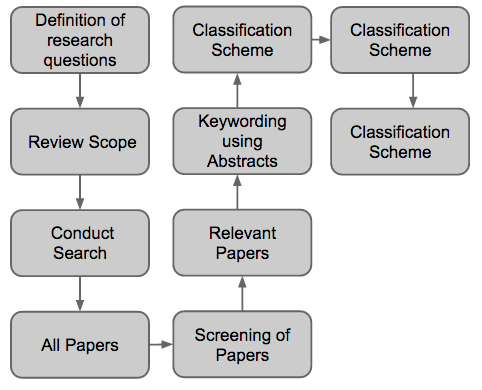
\includegraphics[width=100mm]{Imagens/pic1.png}
\caption{Systematic Mapping Steps~\cite{Petersen:2008:SMS:2227115.2227123}.\label{fig:sms}}
\end{figure}

On the first step, ``Definition of Research question'', the questions that must be answered on the survey are defined. 
On the ``Review Scope'' step, researchers target the papers/journal sources that will be taken into consideration on the systematic map. 
After that, the ``Search'' step is done using a set of predefined search engines and a body of papers (``All papers'') is retrieved. 

After an initial ``Screening of the papers'', the ``Relevant papers'' are chosen according to inclusion and exclusion criteria defined by the research team. 
At this point, the papers that will participate of the study are selected. 
The selection is based on the title, abstracts and keywords of each paper (``Keywording using Abstracts'').

After that, a ``Classification Scheme'' is built, defining different points-of-view (or facets) from which the body of papers will be classified. 
After matching each paper with the classification schema (``Data Extraction and Mapping Process''), the  systematic mapping is performed.
In this phase the relationships between the collected data (in the light of the classification scheme) are used to answer the research questions.




\section{Service Level Agreements (SLAs)}
According to \textit{ITILv3's} official glossary \cite{itilv3glossary}, a Service Level Agreement (SLA) is ``\textit{an agreement between an IT service provider and a customer. 
A service level agreement describes the IT service, documents service level targets, and specifies the responsibilities of the IT service provider and the customer.}'' 

The agreement consists on a set of measurable constraints that a service provider must guarantee to its customers.
In practical terms, it is a document that a service provider delivers to its consumers with minimum quality of service (QoS) metrics. 
If the service is delivered with a lower QoS than is promised on the SLA, consumers may be refunded or earn benefits that were accorded beforehand.    